% texte pour l'introduction générale

Les réacteurs d'avion sont des assemblages complexes de pièces soumises à de
très fortes contraintes. En effet, l'air qui est aspiré à la température 
ambiante, est ensuite compressé dans plusieurs étages de compresseurs, 
avant de rencontrer le kérosène dans la chambre de combustion. Les températures
atteignent alors les \SI{1250}{\celsius}, et l'air est ensuite éjecté du réacteur
et propulse l'avion.


\centerline{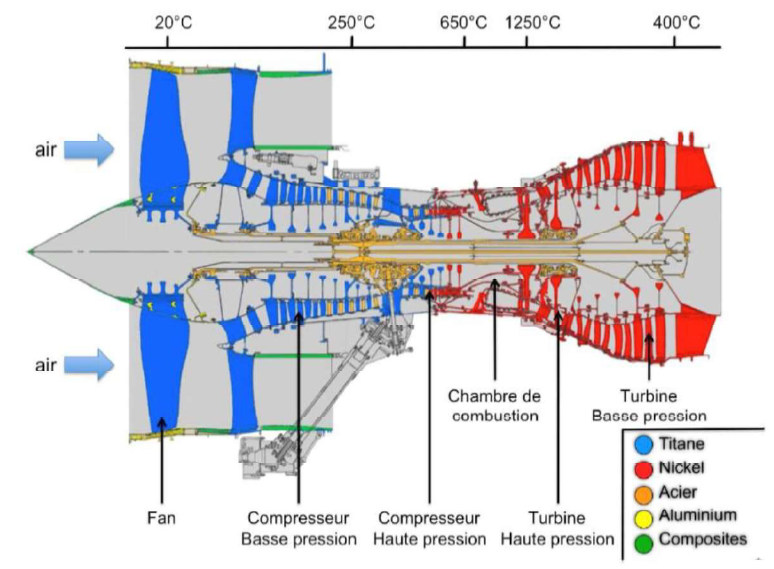
\includegraphics[width=0.55\textwidth]{images/coupe_CFM56.png}}


Les aubes de la turbine haute pression sont ainsi soumises à des conditions très rudes : elle tournent en continu pendant plusieurs heures à $10000$ tours par minute sous une température de 1250°C. C'est pourquoi plusieurs industriels dont Safran cherchent à développer des aubes de turbine résistantes au fluage, notamment grâce à un traitement thermique.


